%\documentclass[wsdraft]{ws-procs11x85}

\documentclass{ws-procs11x85}
\usepackage{ws-procs-thm}           % comment this line when `amsthm / theorem / ntheorem` package is used
\usepackage{multirow}
\usepackage{tabularx}
\newcommand{\etal}{\textit{et al}.}
\newcommand{\TEtranscripts}{\texttt{TEtranscripts}}
\newcommand{\SalmonTE}{\texttt{SalmonTE}}
\begin{document}

\title{Ultra-Fast and Scalable Quantification Pipeline of Transcript Abundances from Next Generation Sequencing Data}

\author{Hyun-Hwan Jeong$^{1,2}$, Hari Krishna Yalamanchili$^{1,2}$, Caiwei Guo$^{2,3}$,Joshua M. Shulman$^{1,2,3}$, and Zhandong Liu$^{2,3,\dag}$}

\address{$^{1}$Department of Molecular and Human Genetics, Baylor College of Medicine,\\
$^{2}$Jan and Dan Duncan Neurological Research Institute, Texas Children’s Hospital,\\
$^{3}$Department of Neuroscience, Baylor College of Medicine,\\
$^{4}$Department of Pediatrics, Baylor College of Medicine,\\
Houston, Texas 77030, USA\\
$^{\dag}$E-mail: zhandonl@bcm.edu}

\begin{abstract}

Transposon elements (TE) are DNA sequences 
that are able to move from a location to another in the genome 
and represent a large proportion (45\%) of human genome. 
% Most of them are not functional, but some of them can be causes of genetic disease. \textit{Needs a better definition.  Please find it textbook and reword} 
% https://www.ncbi.nlm.nih.gov/pmc/articles/PMC3818539/
% Yet, their roles in human health and disease and in genomic evolution are not well defined. Once considered “junk” or “selfish” DNA, TEs are now being appreciated for their specific functional roles in a variety of biological phenomena that can be both beneficial and pathological to the organism (Biémont, 2010)
They are appreciated for their functional roles in a variety of biological phenomena such as
cancer,
neurodegenerative disease, and aging.

Rapid development on RNA-seq technology has enable us, for the first time, to study the activity of TE at systems level .  
However, efficient TE analysis tools are not yet developed.
In this work, we developed \SalmonTE, a fast and reliable pipeline for quantification of TEs from 
RNA-seq data.
Our tool is 20x faster than \TEtranscripts, a benchmark tool in the TE analysis field, when compared using various RNA-seq datasets in Fruit fly and Human cell-line. 
The accuracy of \SalmonTE~on quantifying TEs was validated by RT-qPCR and showed high concordance with existing tools. 
We believe that \SalmonTE~will become a widely used tool to investigate TE expression landscapes from RNA-seq data. 
% Hwan, This is my edit on the abstract, please merge it with Kala's changes. 
% To Zhandong: I replaced abstract to your version

%Transposon elements (TE) are DNA elements which have mobility and represent a large proportion (45\%).
%Most of them are not functional, but some of them can be causes of genetic disease. 
%Rapid development of RNA-seq generates a big genomic data repository and gives a chance for a large-scale study for TE, but 
% * <phamkala@gmail.com> 2017-07-28T18:24:56.789Z:
% 
% > for
% Replace "for" with "of"
% 
% ^ <jeonghyunhwan@gmail.com> 2017-07-28T22:16:04.122Z.
% * <phamkala@gmail.com> 2017-07-28T18:23:21.603Z:
% 
% > of 
% Replace "of" with "for"
% 
% ^.
% * <phamkala@gmail.com> 2017-07-28T18:22:41.759Z:
% 
% Instead of "of" use "for"
% 
% ^ <jeonghyunhwan@gmail.com> 2017-07-28T22:17:16.058Z:
% 
% Kala, did you change it already, if you didn't then could you change it? I can't find where you pointed out.
%
% ^ <jeonghyunhwan@gmail.com> 2017-07-28T22:18:43.088Z:
% 
% I think it must be "Rapid development of RNA-seq generates a big genomic data repository and gives a chance for a large-scale study for TE, but ", right?
%
% ^.
%no feasible TE analysis tools are out yet.
%In this work, we have developed \SalmonTE, a fast and reliable pipeline for quantification of TEs from 
%Next Generation Sequencing (NGS) data.
% * <phamkala@gmail.com> 2017-07-28T18:26:23.109Z:
% 
% > NGS
% Not sure if you specified early, but what is NGS? Does it stand for Next Generation Sequencing Data? If so,  replace "NGS" with "Next Generation Sequencing  (NGS)" so that it is clear. After this, you can use NGS wherever you want and it will be clear that you are talking about Next Generation Sequencing. 
% 
% ^ <jeonghyunhwan@gmail.com> 2017-07-28T22:14:55.653Z:
% 
% It is fixed. Thanks.
%
% ^.
%The demonstration of \SalmonTE~for the various datasets has shown a dramatical speed-up compared to \TEtranscripts, 
% * <phamkala@gmail.com> 2017-07-28T20:11:31.823Z:
% 
% > the
% Change to "a"
% 
% ^.
% * <phamkala@gmail.com> 2017-07-28T20:08:50.667Z:
% 
% > comparing
% Change to "compared"
% 
% ^.
%and the comparison of counts and fold-changes to the previous method and RT-qPCR has shown this pipeline can 
%provide an precise quantification result for a given input dataset. 
% * <phamkala@gmail.com> 2017-07-28T20:12:00.410Z:
% 
% Maybe add "a" before "given"
% 
% ^.
%We conclude this pipeline will be the first starting point which enables a large-scale TE study.
\end{abstract}

\keywords{Transposon Element; Quasi Mapping; RNA-seq; Next Generation Sequencing; Large Scale Genome Analysis}

% required
\copyrightinfo{\copyright\ 2017 The Authors. Open Access chapter published by World Scientific Publishing Company and distributed under the terms of the Creative Commons Attribution Non-Commercial (CC BY-NC) 4.0 License.}

% required
\bodymatter

\section{Introduction}\label{aba:intro}

Transposon elements (TE) are DNA elements which can be mobilized or inserted into the genome and represent a significant proportion (45\%) of most eukaryotic genomes \cite{erwin2014mobile}. 
% The first observation of TEs was in \textit{Zea Mays (maize)} by Barbara McClintock in 1948 \cite{McClintock01011951}. 
Most of the TEs in genome are not functional and had been considered as `junk DNA,' except a few has intact functions such as transcription and mobilization.\cite{biemont2006genetics}
Furthermore, the mobilization of TEs can disrupt normal gene strcuture in the genome can cause a few genetics diseases including cancer \cite{belancio2008mammalian} such as cancer,
\cite{jirtle2007environmental}
neurodegenerative diseases,\cite{erwin2014mobile} and aging.\cite{wood2013chromatin} % citations!

Recent development of high-throughput Next Generation Sequencing (NGS), like RNA-seq
enables genome wide study for TEs [\refcite{ohtani2013dmgtsf1,mihevc2016tdp,li2012transposable,krug2017retrotransposon}], and several algorithms and pipelines were proposed to analysis reads files from TE studies \cite{lee2012landscape,platzer2012te,helman2014somatic,henaff2015jitterbug,jin2015tetranscripts,de2017identifying,tang2017human}. However, most of the tools share some common limitations: 1) Discordant read mapping, due to chance of multiple mapping is much higher in repetetie elements shared by TEs in the same clade, 2) limited scalability for large-scale analysis, and 3) small coverage for the entire TEs defined in human genome. For example, a tool used in [\refcite{tang2017human}] only consider LINE 1 (Long Interspersed Nuclear Element 1) element.
\cite{ewing2015transposable} 
Among the existing tools, \TEtranscripts~is reported this tool resolves most of the issues and has performed well in various datasets.
\cite{jin2015tetranscripts}
Nonetheless, The scalability of \TEtranscripts~is a critical limiting factor for large systems biology studies because this tool cannot handle \verb|FASTQ| file directly and needs \verb|SAM|(Sequence Alignment Map)/\verb|BAM| (Binary Sequence Alignment Map) files generated from raw \verb|FASTQ| files to execute \TEtranscripts. Since there are many tuning parameters on handling repetitive sequence mapping among different RNAseq mapping algorithms, this step will be highly variable depending on the mapping parameters and sometimes even generate artificial results if a unique mapping paramer was superimposed by a previous analyst who handled the mapping. 
Furthermore, the interval tree algorithm \cite{samet1990design}, which is used to find interval of genes or TEs on reference genome,  performed poorly in terms of running time in practice. Thus, \TEtranscripts~is not a feasible tool to perform large-scale TE analysis.

Although most of TE studies contains a few RNA-seq samples, recent studies demonstrated that large-scale analysis of public meta RNA-seq datasets offered new insight and
findings that cannot be discovered in each individual dataset. \cite{nellore2016human} However, a meta study on TE without using a large number of high performance computing cluster is not yet feasible given the time complexity of current algorithms.  To achieve this, we developed a new pipeline \SalmonTE. It deploys an low time-complexity quantification methods of \verb|Salmon|\cite{patro2017salmon} and contains various statistical analysis for the quantifications. Moreover, user do not have to do any pre-processing for their raw \verb|FASTQ|. 
In the results section, we demonstrate that the running speed of  \SalmonTE~outperforms \TEtranscripts~and delivers a reliable quantification result as well.

\section{Methods}

The proposed pipeline consists of three parts: library preparation, quantification, and statistical analysis (Figure \ref{aba:fig1}). 
The entire source codes and executable scripts are available at \url{https://github.com/hyunhwaj/SalmonTE}. 
% Is it better to say "three parts" than "two parts?"

\begin{figure}[!ht]
\centerline{
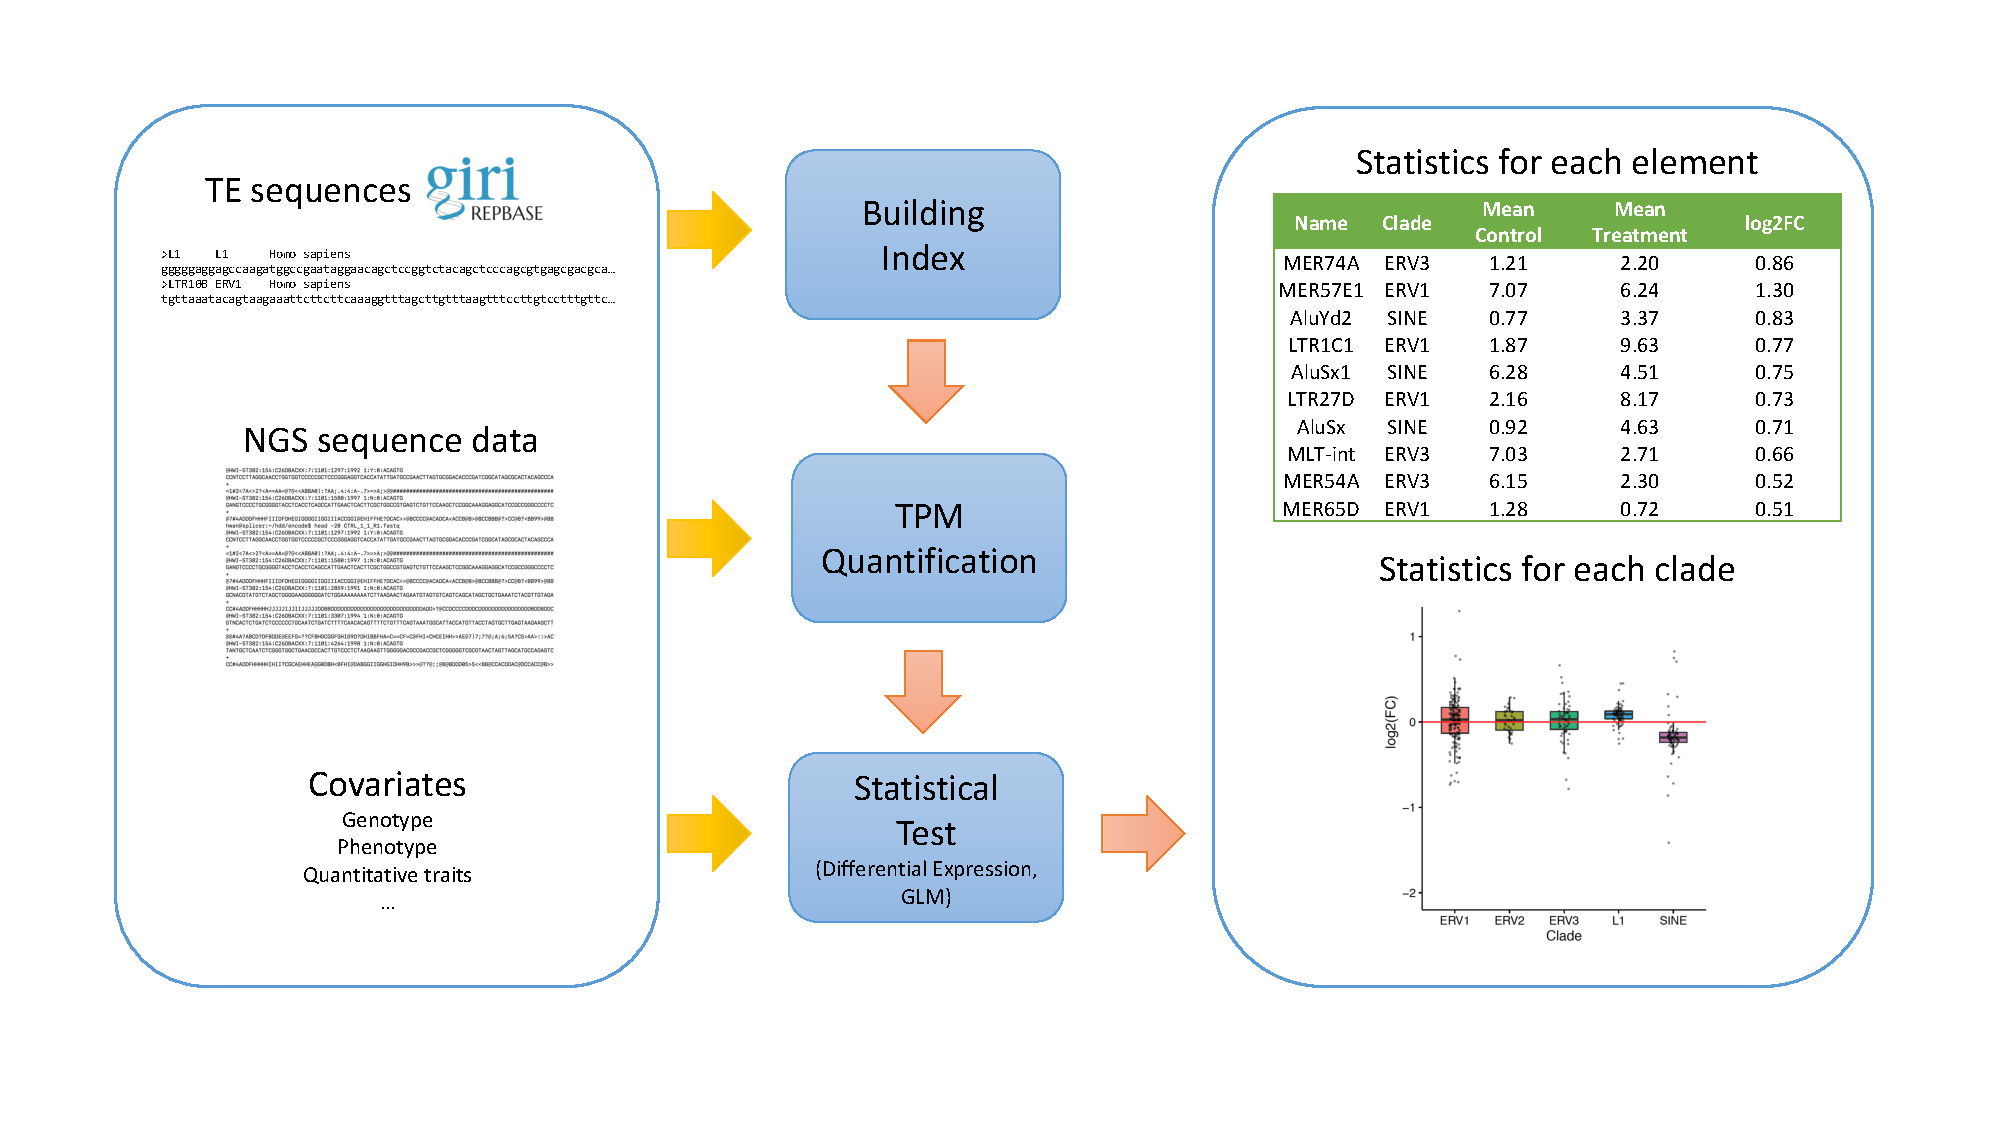
\includegraphics[width=16cm]{fig1.pdf}
}
\caption{An illustration of the \SalmonTE~pipeline.}
\label{aba:fig1}
\end{figure}

\subsection{Transposon Element Library Preparation}
We collected the consensus cDNA sequence library of TEs for \textit{Homo Sapiens} and \textit{Drosophila Melanogaster} from Repbase  
(version 22.06)\cite{repbase}. We did not include cDNA sequences of simple repeats and multicopy genes, and DNA transposons (which replicate without an RNA intermediate). 
Next, we manually curated clades of each TE, based on the annotation of Repbase. As a result, our library contains 687 TEs for \textit{Homo Sapiens} and 163 TEs for \textit{Drosophila Melanogaster}.

\subsection{Salmon quantification algorithm}
We adopted the \verb|Salmon| [\refcite{patro2017salmon}] algorithm to quantify the transposon elements abundance from given RNA-seq reads files. \verb|Salmon| enables a fast and accurate quantification of transcript expression from RNA-seq reads with quasi-mapping, a variant of stochastic, collapsed variational Bayesian inference(in the online phase), and Expectation Maximization (EM) algorithm (in the offline phase)
\cite{patro2017salmon,srivastava2016rapmap,bishop2006pattern,foulds2013stochastic}. 
%We describe details of algorithms and models uses in \verb|Salmon| in this section.

Before running online and offline inference on the counts of each transposon elements from a given reads file,
Salmon runs a quasi-mapping which is initially proposed in [\refcite{srivastava2016rapmap}]. A quasi-mapping specifies the target of each given read and also determines the position and the orientation of the read concerning the target by computing the
Maximum Mappable Prefix (MMP) [\refcite{li2012exploring}] and Next Informative Position (NIP) [\refcite{srivastava2016rapmap}] of the read.
This mapping procedure depends on a generalized suffix array \cite{manber1993suffix}, 
and it enables a fast and accurate mapping as compared to other mapping tools, such as \verb|Bowtie 2|, \verb|STAR|, and \verb|Kalisto| \cite{srivastava2016rapmap}. 

The online phase is to model the conditional probability $Pr \{f_j | t_i \}$, and
uses the following auxiliary terms:

\begin{equation}
Pr \{f_j | t_i \} = Pr \{ l | t_i \} 
\cdot Pr \{ l | t_i \} 
\cdot Pr \{ p | t_i, l \} 
\cdot Pr \{ o | t_i \} 
\cdot Pr \{ a | f_j, t_i, p, o, l \} 
\end{equation}

% better to rephrase
where $Pr \{ l | t_i \}$ 
is the probability of drawing a read of the inferred length $l$ given $t_i$,  
$Pr \{ p | t_i, l \}$ is the probability of the read starting at position $p$ on $t_i$,
$Pr \{ o | t_i \}$ is the probability of obtaining a read
alignment with the given orientation $o$ to $t_i$, and
$Pr \{ a | f_j, t_i, p, o, l \} $ is the probability of the alignment $a$ \cite{patro2017salmon}. 
This model accounts for sample-specific parameters and biases.
Laissez-faire stochastic variational Bayes SCVB0 inference algorithm is used to 
compute the online abundance estimates auxiliary model parameters\cite{patro2017salmon}.

After the quasi mapping, 
we can estimates abundance (reads count) of each TEs. 
Suppose that
we have $M$ TEs and the set of underlying true TE cunts are given as
$T = \{(t_1, \dots , t_M), (c_1, \dots, c_M) \}$, where $t_i$ is the nucleotide sequence of $i$-th transcript in the set and $c_i$ is true count of the corresponded transcript. 
If $T$ contains a complete counts then we can calculate the nucleotide fraction \cite{li2009rna} of each $t_i$ from (\ref{eq:1}).
 

\begin{equation} \label{eq:1}
\eta_i = \frac{c_i \cdot \widetilde{l_i} }{\sum_{j=1}^{M} c_j \cdot \widetilde{l_j}}
\end{equation}

In (\ref{eq:1}), let $\widetilde{l_i}$ denote the effective transcript length of $t_i$\cite{li2009rna}.

We also can calculate the transcript fraction of each transcript from (\ref{eq:2}).

\begin{equation} \label{eq:2}
\tau_i = \frac{ \frac{\eta_i }{\widetilde{l_i}} }
{\sum_{j=1}^{M} \frac{\eta_j }{\widetilde{l_j}} }
\end{equation}

$\tau_i$ can be used a measure of relative transcript abundance.

With $\tau_i$, Transcripts Per Million (TPM) calculated as $TPM=\tau_i \times 10^6$ and the $TPM$ uses as a relative abundance measure of each transposon element for a given sample in this study.

To estimate $T$, the maximum likelihood approach is used to assess given $T$ and $F$ which is a given set of mapped sequence reads from 
the online inference step.
We can define the probability of observing a set of sequenced fragments as below,

\begin{equation} \label{eq:3}
Pr\{F|\eta,Z, T \}=
\prod_{j=1}^{N}\sum_{i=1}^{M} Pr\{ t_i | \eta \}  \cdot
 Pr \{ f_i | t_i , z_{ij} = 1 \}
\end{equation}

where $z_{ij} = 1$ denotes if $j$-th read in $F$ is derived from transcript $i$. The likelihood objective can be optimized using EM algorithm \cite{li2009rna}.

To increase the usability and enable parallel processing for multiple RNA-seq reads files, we adopted \verb|Snakemake| workflow system and wrote a script on the execution rule for \verb|Snakemake|.\cite{koster2012snakemake}
% Still completing pipeline, and it will out to github and our website.

\subsection{Statistical tests}
We provided a statistical analysis function to identify differential expressed TEs from the counts table as the last step of the pipeline. 
Differential analysis using DEseq2 can handle  binary covariates such as binary genotype, phenotype and gender \cite{love2014moderated}. We can also apply General Linear Model (GLM) for quantitative covariates such as disease pathology score and age \cite{johnston1980multivariate}. The analysis will make two different outputs, 
the first one is the test statistics for each TE, and the second one is the summary of the statistics for each clade. 
The output files are provided with various file formats, such as tab-separated values file (TSV), XML spreadsheet file format (XLS, XLSX), R object file (Rdata), and Portable Document Format (PDF) file.

\section{Results}

\subsection{Experiment setup}
In the paper of \TEtranscripts, they demonstrated that \TEtranscripts~is the best method among the published methods in terms of recovery accuracy of TE and running time for both cases of a synthetic dataset and published data. 
Thus, we only compare performance of our pipeline to \TEtranscripts. 
The RNA-seq data used in [\refcite{ohtani2013dmgtsf1}], is from Gene Expression Omnibus (accession no. GSE47006), which were also used in the \TEtranscripts~paper, 
were used to compare performance of running time and quantification accuracy between
our proposed pipeline and \TEtranscripts.
As a pilot study, we seek to identify TEs that are  differentially express between ALS (Amyotrophic Lateral Sclerosis)  patients and healthy  controls.
We demonstrated our pipeline with a K562 cell-line RNA-seq dataset from ENCODE (Encyclopedia of DNA Elements, \url{http://encodeproject.org}) [\refcite{encode2012integrated}] Consortium (accession ID: ENCBS555BYH). 
The dataset consists of two biological replicates of shRNA (short hairpin RNA) knockdown (KD)
targeting \textit{TARDBP} (TAR DNA Binding Protein, as known as TDP-43) gene and two biological replicates of controls 
(a shRNA inserted but targets no genes). 
It has been reported that loss of \textit{TDP-43} function causes phenotypes of 
ALS.\cite{yang2014partial,mihevc2016tdp} To measure scalability with the dataset
we also ran \TEtranscripts~to compare running time of both methods.


Generating BAM files from \verb|FASTQ| files are mandatory to use \TEtranscripts, so we applied \verb|STAR| [\refcite{dobin2013star}] to generate the files with following parameters
\verb|--outFilterMultimapNmax 100| and \verb|-–winAnchorMultimapNmax 100|. We also used 16 threads for the both \SalmonTE~and \verb|STAR|(for \TEtranscripts).
All of computational experiments in this work was done in a workstation with 
\verb|Intel(R) Xeon(R) CPU E5-2630 v4 @ 2.20GHz| (has 10 cores and maximum 40 threads) and \verb|128GBytes| RAM.


\subsection{Performance Benchmark on \SalmonTE}

%Table \ref{aba:table1} shows a summary of the datasets used in the experiments and indicates the result of measuring the runtime of \SalmonTE~and \TEtranscripts~for both datasets. 
Compared to \TEtranscripts~,  \SalmonTE~ showed a 19x to 27x fold increase in speed (Table \ref{aba:table1}).

In this analysis, we observe that \SalmonTE~outperforms \TEtranscripts~regarding processing speed, and this pipeline just took less than 5 minutes for a sample, while \TEtranscripts~needs about 2 hours to process a single sample. 
It also demonstrates \SalmonTE~can easily handle thousands of samples if the pipeline is extended using a cloud service. 
Table \ref{aba:table_amazon} shows 
our estimated cost if the proposed pipeline were implemented in a cloud computing environment, and it predicts the price is 22 times less than  less than using \TEtranscripts.  

\begin{table}[h]
\tbl{Performance comparison between \SalmonTE~and \TEtranscripts.}
{
\begin{tabular*}{.8\textwidth}{@{\extracolsep{\fill}}llll}
\hline
Dataset                          & Piwi KD [\refcite{ohtani2013dmgtsf1}]    & K562 \textit{TDP-43} \\ \hline
Total number of samples          & 2          & 4             \\ 
RNA-seq file type                & Single end & Paired ends  \\ 
Total number of reads            & 90,411,467 & 309,701,182   \\ \hline
\SalmonTE~runtime (hh:mm:ss)      & 0:05:33    & 0:17:13       \\
\TEtranscripts~runtime (hh:mm:ss) & 1:45:26    & 7:49:40       \\
Speedup                          & 19.00x     & 27.28x        \\ \hline
\end{tabular*}}\label{aba:table1}
\end{table}

\begin{table}[h]
\tbl{Price estimation of both \SalmonTE~and \TEtranscripts~in cloud computing environment (Amazon Elastic Compute Cloud (EC2),
and Amazon Elastic Block Store (EBS)). We assume that size of \texttt{FASTQ} file for a sample is 20GB for the calculations.}
{\begin{tabular}{lrr}
\hline
Methods & \SalmonTE~& \TEtranscripts \\ \hline
Estimated total running time for 1000 samples & 90 hours & 2,000 hours \\ 
The price of Amazon EC2 (m4.10xlarge, US Oregon region) [\refcite{ec2}] & \$180 & \$ 4,000 \\
The price of Amazon EBS (gp2 40TB, US Oregon region) [\refcite{ebs}] & \$500 & \$ 11,111 \\  
Total price & \$680 & \$ 15,111 \\ \hline
\end{tabular}}\label{aba:table_amazon}
\end{table}

\subsection{Quantification Accuracy}

\begin{figure}[h]
\centerline{
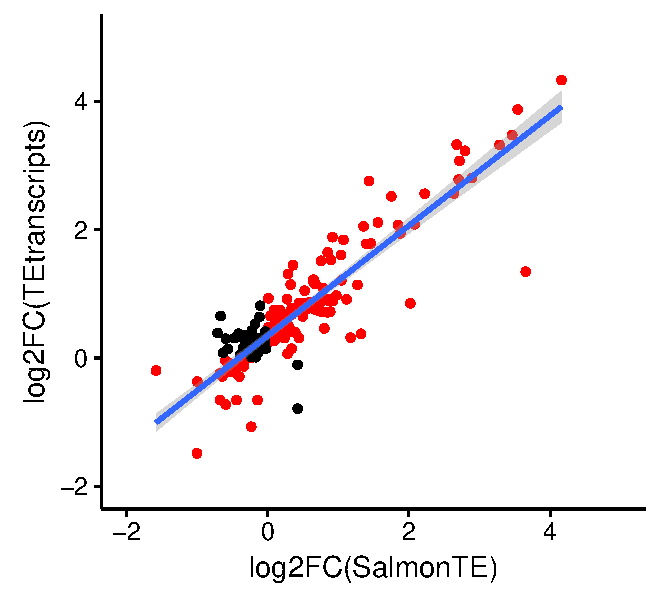
\includegraphics[width=11cm]{figure_corr_FC}
}
\caption{Correlation of $log_{2}FC$ ($\frac{Piwi}{WT}$) for each transposon element between \SalmonTE~and \TEtranscripts. Red points represents points with same fold change direction between \SalmonTE~and \TEtranscripts.}
\label{aba:fig2}
\end{figure}

First, we compared the estimated $log_{2}FC$ of \SalmonTE~and \TEtranscripts~on each transposon element from Ohtani \etal's data. 
Figure \ref{aba:fig2} shows that the estimated TE abundance of both methods are highly correlated ($r^{2}=0.98$), and we also observed there is a high concordance in the direction of fold-changes between \SalmonTE~and \TEtranscripts. We also measured the correlations of normalized read counts between \SalmonTE~and \TEtranscripts, 
and we can see that the calculated read counts from those methods are highly correlated in each sample. ($r^2=0.92$ for wild-type (WT) sample and $r^2=0.91$ for PiWi KD sample).
From this observation, we conclude that \SalmonTE~has similar as  \TEtranscripts~accuracy in TE quantifcation.

\begin{figure}[h]
\centerline{
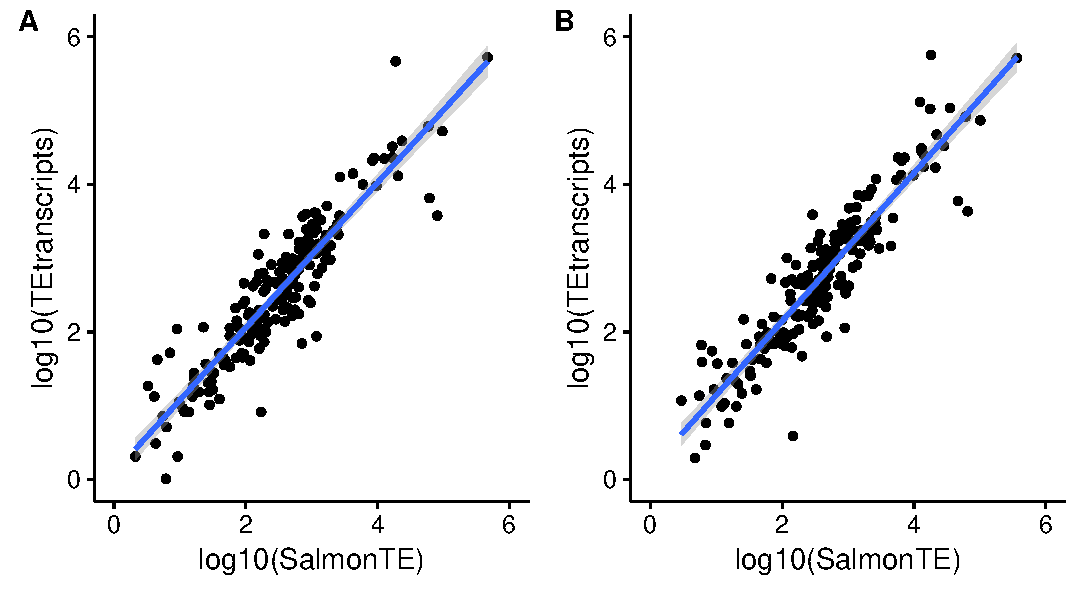
\includegraphics[width=13cm]{figure_corr_count}
}
\caption{Sample correlation of count for each transposon element between \SalmonTE~and \TEtranscripts. \textbf{A}. WT sample, \textbf{B}. PiWi KD sample.}
\label{aba:fig3}
\end{figure}

Next, we took 8 TEs which were quantified by
Reverse Transcription-quantitative Polymerase Chain Reaction (RT-qPCR)
and validated with measuring the correlation of $log_{2}FC$ on each selected TE between RT-qPCR and \SalmonTE.
We observed a high correlation between \SalmonTE~and RT-qPCR on those elements ($r^2=0.97$, Figure \ref{aba:fig4}). 

\begin{figure}[h]
\centerline{
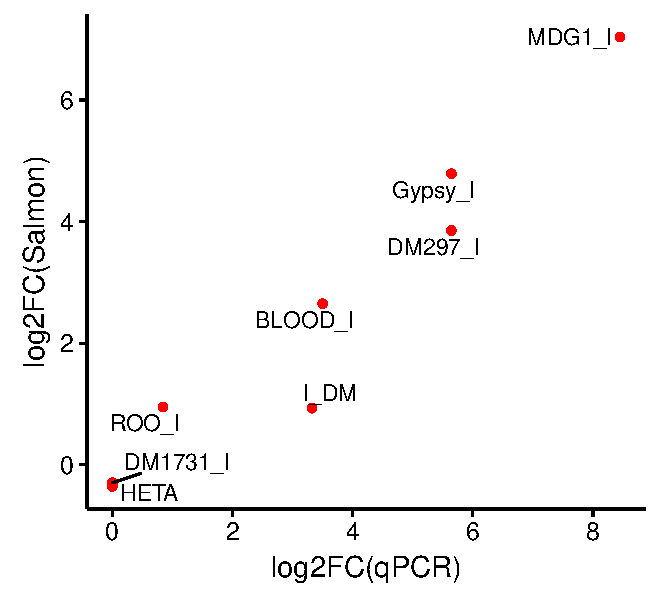
\includegraphics[width=10cm]{supp_fig3_corr}
}
\caption{Comparison between \SalmonTE~and RT-qPCR}
\label{aba:fig4}
\end{figure}

\subsection{Demonstration on K562 cell-line TDP-43 data}

Finally, we applied \SalmonTE~pipeline to a \textit{TARDBP}(TAR DNA Binding Protein, as known as TDP-43) knockdown in human cell line. 
We identified 23 transposon elements that are differential expressed between TARDBP knockdown and control cell lines (Table \ref{aba:table2}) with $|log_{2}FC| \geq 0.5$. 
We can see that most of the differentially expressed features are Endogenous Retrovirus (15 of 23) in \textit{TDP-43} cell-line sample, and 
we hypothesize that some of differentially Endogenous Retrovirus TEs are associated with ALS.

% we may need to the interpretation
To identify if there is any general differential expression trend on subfamiles of TE, we grouped all the TEs based on their clade information in Repbase. We excluded all of the CR1 (Chicken Repeat 1) since the number of such elements in the clade is small.
We found that SINE (Short Interspersed Nuclear Elements) are mostly down expressed,
and elements in L1 (Long interspersed nuclear element 1) are generally over expressed in TARDBP knockdown samples. 
This result provides a working hypothesis that knocking-down of \textit{TDP-43}  repress the expression of SINE elements and induce the expression of L1 elements.

\begin{table}[h]
\tbl{23 Differentially expressed transposon elements in the ENCODE TARDBP data}{
\begin{tabular*}{.5\textwidth}{@{\extracolsep{\fill}}ccc}
\hline
Name & Clade & log2FC\\
\hline
MER74A & ERV3 & 1.68\\
MER57E1 & ERV1 & 1.30\\
AluYd2 & SINE & 0.83\\
LTR1C1 & ERV1 & 0.77\\
AluSx1 & SINE & 0.75\\
LTR27D & ERV1 & 0.73\\
AluSx & SINE & 0.71\\
MLT-int & ERV3 & 0.66\\
MER54A & ERV3 & 0.52\\
MER65D & ERV1 & 0.51\\
LTR28 & ERV1 & -0.59\\
LTR1F & ERV1 & -0.63\\
FLAM & SINE & -0.64\\
MER21 & ERV3 & -0.68\\
MER101 & ERV1 & -0.69\\
LTR26B & ERV1 & -0.70\\
MER83C & ERV1 & -0.71\\
AluJo & SINE & -0.72\\
LTR06 & ERV1 & -0.73\\
MLT2D & ERV3 & -0.78\\
AluYf5 & SINE & -0.86\\
AluYd3 & SINE & -1.41\\
THER2 & SINE & -2.03\\ \hline
\end{tabular*}}\label{aba:table2}
\end{table}


\begin{figure}[h]
\centerline{
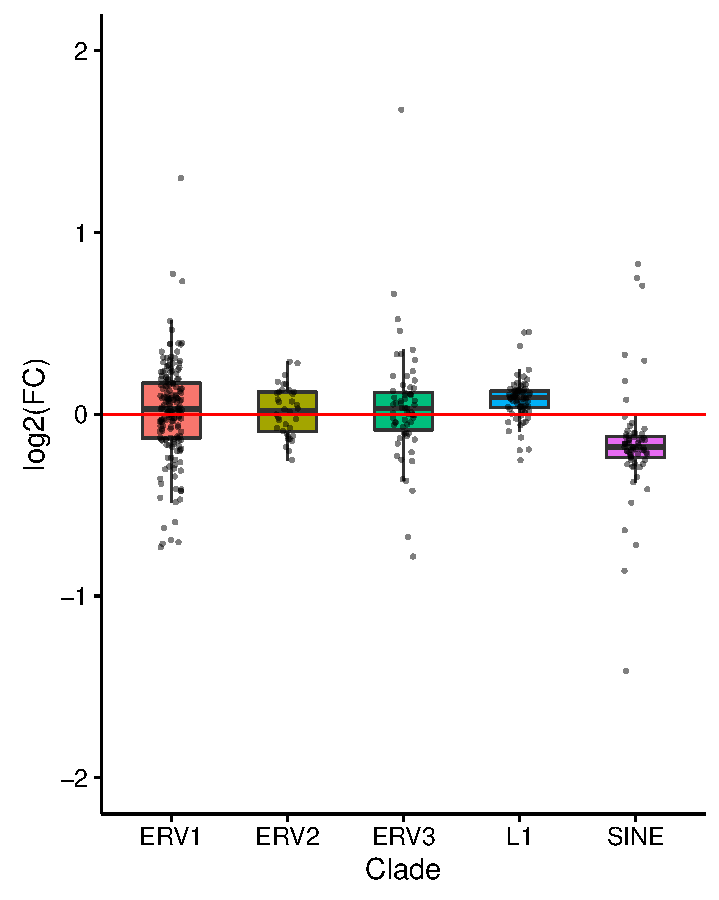
\includegraphics[width=10cm]{boxplot-clade-k562}
}
\caption{An boxplot of $log_{2}FC$ for each clade in the ENCODE TARDBP data}
\label{aba:fig5}
\end{figure}

\section{Conclusion}


In this work, we  developed \SalmonTE, a fast and reliable pipeline for quantification of TEs from 
NGS data.
Our comparison results of \SalmonTE~on the various datasets has shown a dramatical speed-up in computing time relative to \TEtranscripts, 
and
an accurate quantification on TEs. 
Therefore, we expect this pipeline will enable the biomedical research community to re-analyze the large amount of data generated over the past few years from the angle of TE expression. 

There are still several remaining features need to be implemented in the future to improve the usability of \SalmonTE. 
For example, prediction of genomic locations which 
contain the differentially expressed TEs is highly needed in many TE studies. Several methods was developed toward this end\cite{de2017identifying,criscione2014transcriptional}, but these tools share the scalability issue and require
massive computing power for a large-scale TE study. 
Alignment free algorithms are intrinsically limited in address this 
question. 
%Developing a novel pipeline for the prediction with alignment free quantification manner which uses in \SalmonTE~
%resolves the issue, but currently developed alignment-free methods such as \verb|Sailfish| \cite{patro2014sailfish}, \verb|Salmon|\cite{patro2017salmon}, 
%and Kalisto \cite{bray2015near} are limited to use
%because the genomic information of TEs is not prior information to be considered in those methods.
Therefore, we foresee a novel algorithm which extends and improve a current alignment-free method needs to be developed to address this.

\section*{Acknowledgments}

\bibliographystyle{ws-procs11x85}
\bibliography{ws-pro-sample}

\end{document}